\section{Comparison to a CUDA implementation}
We compared our implementation of forward projection and back projection to implementations from the astra toolbox. However we only compared the algorithms through python, by compiling our algorithms with pyopencl and running them through python and doing the same with the forward and backward rpojection from the atsra toolbox. Ideally the functions should have been compared without the memory overhead.
\begin{figure}[h]
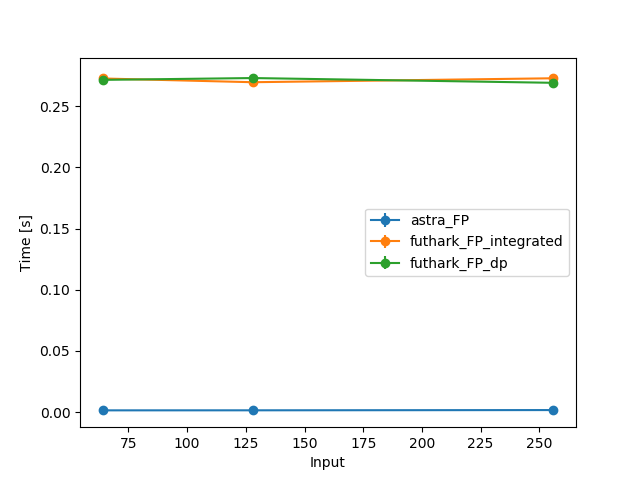
\includegraphics{images/FPplot.png}
\end{figure}
\begin{figure}[h]
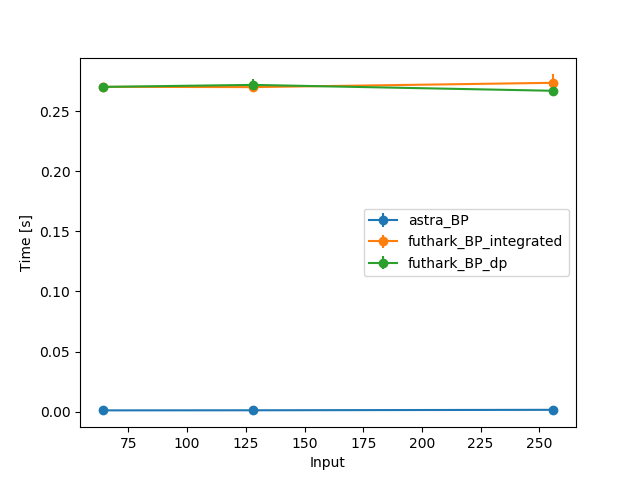
\includegraphics{images/BPplot.png}
\label{astra}
  \caption{A comparison of the back projections from astra and our fastest futhark algorithms. The futhark algorithms perform much worse, approximately 128 times worse for both forward and backprojection. It would be worth comparing our code with the implemented version from the astra toolbox, to see how they get such a good running time.}
\end{figure}
